\section{System requirement}
This research aims to improve the security of smart device (especially the smart sensor) in IoT system. 
The security system we want to implement must have the following requirements. 

\begin{enumerate}
    \item \textbf{Guarantee device safety;} The focus of the system is to secure the perception layer of IoT system, the sensor.  
    \item \textbf{Independent from device;} System should be able to operate without any additional setups on IoT devices. This design help reducing the additional work when dealing with a large-scaled IoT system.    
    \item \textbf{Can implement on top of an existed system;} Users can easily install system without having to change their network topology.
    \item \textbf{Do not affect system performance;} After system is added to the workspace, it should not impede on the performance: system latency, packet drop.
    \item \textbf{Reduce system manager’s task; } Normally, the system manager can investigate the system integrity by looking its traffic pattern, system performance, CPU temperature and more. However, considering that system manager can come and go, without well written document, it is quite burdensome for user, or new manager to understand the system by themselves. We believe that the system must perform partially automatic without any help from user.
\end{enumerate}

\begin{figure}
    \centering
    \begin{subfigure}[b]{0.4\textwidth}
        \centering
        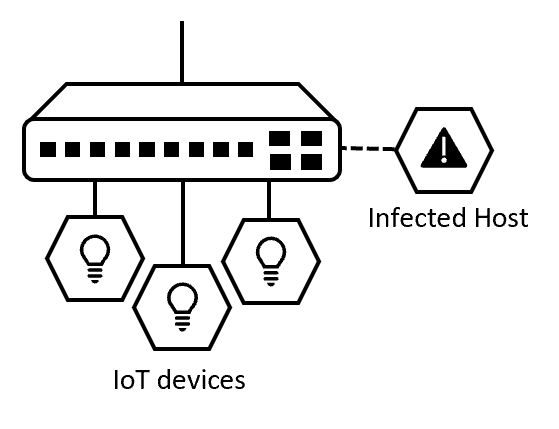
\includegraphics[width=\textwidth]{1_lan}
        \caption{LAN Level Security}
        \label{fig:s3_lan} 
    \end{subfigure}
    \hspace{1.5cm}
    \begin{subfigure}[b]{0.4\textwidth}
        \centering
        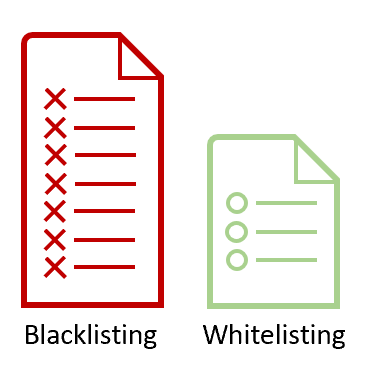
\includegraphics[width=\textwidth]{1_whitelist}
        \caption{Whitelist}
        \label{fig:s3_whitelist}
    \end{subfigure} 
    \caption{System's key characteristics}
    \label{fig:s3_system_characteristics}
\end{figure}


\section{Idea behind the proposed system}
 
We wanted to create the system with all characteristics mention above. The approach we came up consists of two main idea: Switch level security and Whitelist.  

\subsection{Switch level security}
Switch level security is securing IoT at the lower level of network protocol. The security measurement is done outside of the edge device, between the internet and device. (figure \ref{fig:s3_lan}) The benefit of using this method is that there is no need for additional configuration at edge devices. Moreover, it is security at low level where transmission protocol is more restricted, therefore can be managed more easily. Another benefit of layer 2 security is even when malicious host or infected host has entered the local area network, it can prevent the infection from spreading. 

\subsection{Whitelist}
Consider that the number of hosts, sensor normally connect to is limited: NTP (Network Time Protocol) server for clock synchronization, DNS (Domain Name System) Server for translating between host name and IP address, DHCP (Dynamic Host Configuration Protocol) server for dynamic IP assigning, HTTP (Hypertext Transfer Protocol) server for its application usage and vender specific communication protocol. Whitelist approaching is considerably more ideal in IoT sensor.

\section{System Architecture}
\begin{figure}[h]
    \centering 
    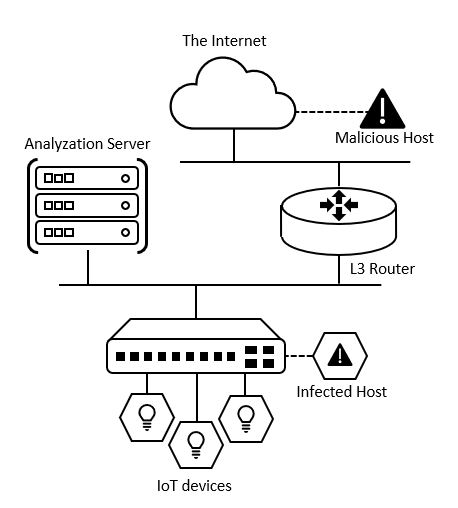
\includegraphics[width=0.6\textwidth]{2_system_architecture}
    \caption{System Architecture }
    \label{fig:s3_system_architecture} 
\end{figure}

System operation is divided into 3 stages: Preparation stage, Analyzation stage and Operation stage. Preparation stage and Analyzation stage would be performed at the system’s initialization, while Operation stage is used after that for the rest of system operating period.  

\subsection{Preparation Stage}
In this stage, all packet going through switch would be captured. This system is developed under the assumption that during Preparation Stage, the network, edge devices, servers, middleware is secure and no malicious software has entered into the system yet.

\subsection{Analyzation Stage}
In Analyzation stage, data collected by network plane is then further investigated to find.  
\begin{enumerate}
    \item All devices in the LAN, \textbf{Host discovery}.
    \item All hosts, each device needs to operate, \textbf{Whitelist Extraction}. 
\end{enumerate}

\subsubsection{Host Discovery}
We believe that it is possible to find all devices in LAN by analyzing captured ARP (Address Resolution Protocol) packets.

\subsubsection{Whitelist Extraction}
Whitelist Extraction program use packet data to create whitelist profile for each discovered host. In this research, we use rule-based algorithm to extract whitelist.

\paragraph{Definition of Secured host and Whitelist Rule}
In this research, we define secure host as “host that device needs in order to fully operate” and we assume that secure host can be extracted using the following rule.  

\subparagraph{}
\begin{centering}
    \textit{“Only IP addresses to which the device initiates connection is considered secured host”} \\
\end{centering} 

\subsection{Operation Stage}
After Analyzation Stage, switch would start filtering network traffic, letting device to only communicate with hosts in its whitelist, guarantee the integrity of IoT system. 

\subsection{System Operation Flow}
\begin{figure}[h]
    \centering 
    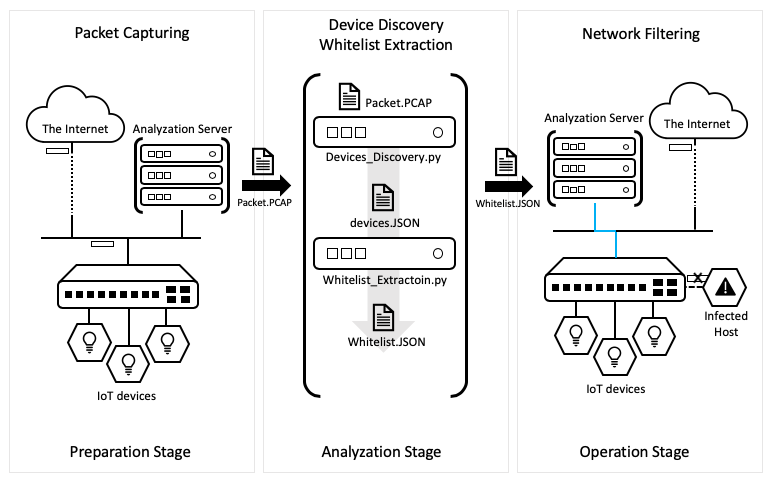
\includegraphics[width=1.0\textwidth]{3_overview}
    \caption{System Overview}
    \label{fig:s3_system_overview}
\end{figure}

First, we start capture devices’ packet under assumption that there is no on-going attacks or infected host in the LAN. After packet data is sufficiently captured, we pass gathered packet to analyzation server, where packet is inspected to find devices in the system. Then we create a whitelist for each device and start filtering traffic according to it. 